\documentclass{beamer}
\usepackage[utf8]{inputenc}
\usepackage[T1]{fontenc}
\usepackage[english]{babel}
\usepackage{graphicx}
\usepackage{times}
\usepackage[normalem]{ulem}
\usepackage{enumerate}
\usepackage{listings}
\usepackage{mathtools}
\usepackage{amsmath}
\usetheme{AGH}

\title[Inicjalizacja tła]{Metody Inicjalizacji modelu tła}

\author[J.Gola, Z.Tekiela]{Jakub Gola, Zbigniew Tekiela }

\date[2012]{22.11.2012}

\institute[AGH-UST]
{Wydział EAIiIB\\ 
Informatyka Stosowana
}

\setbeamertemplate{itemize item}{$\maltese$}

\begin{document}

{
%\usebackgroundtemplate{
\includegraphics[width=\paperwidth]{titlepage}} % wersja angielska
\usebackgroundtemplate{
\includegraphics[width=\paperwidth]{titlepagepl}} % wersja polska
 \begin{frame}
   \titlepage
 \end{frame}
}

%---------------------------------------------------------------------------
\begin{frame}
\begin{center}
\Huge{Metody przestrzenne}
\end{center}


\end{frame}

%---------------------------------------------------------------------------

\begin{frame}
\frametitle{Metody przestrzenne}
\begin{block}{Założenia}
\begin{itemize}
\item Obliczenia są wykonywane na kwadratowych blokach
\item Tłem zostaje najczęściej powtarzający się blok
\item Do dobrania najlepszego bloku jest używana transformata operująca w dziedzinie częstotliwości
\end{itemize}
\end{block}


\end{frame}
%---------------------------------------------------------------------------
\begin{frame}
\frametitle{Metody przestrzenne}
\begin{block}{Fazy algorytmu}

\begin{enumerate}
\item Kolekcjonowanie kandydatów
\item Częściowa rekonstrukcja tła
\item Końcowa rekonstrukcja tła z wykorzystaniem transformaty
\end{enumerate}
\end{block}


\end{frame}
%---------------------------------------------------------------------------
\begin{frame}
\frametitle{Metody przestrzenne}
\begin{block}{Kolekcjonowanie kandydatów}

\begin{enumerate}
\item Podziel ramkę na bloki
\item Dla każdego bloku wykonaj
	\begin{enumerate}
	\item Jeśli to pierwszy blok, dodaj go do zbioru reprezentantów
	\item Jeśli to kolejny blok, porównaj go z każdym innym w zbiorze reprezentantów
		\begin{itemize}
		\item Jeśli znajdziesz wystarczająco podobny blok, uaktualnij go
		\item W przeciwnym wypadku dodaj blok do zbioru reprezentantów
		\end{itemize}
	\end{enumerate}
\end{enumerate}
\end{block}


\end{frame}
%---------------------------------------------------------------------------
\begin{frame}
\frametitle{Metody przestrzenne}
\begin{block}{Kryteria podobieństwa bloków}
\begin{equation}
\label{Tcorr}
T_{corr}=\frac{{(r_k(i,j)-\mu_{r_k}(i,j)}^T(b_f(i,j)-\mu_{b_f})}{\sigma_{r_k}\sigma_{b_f}}
\end{equation}
\begin{equation}
T_{MAD}=\sum_{n=0}^{N^2-1}\left|b_{f_n}(i,j)-r_{k_f}(i,j)\right|
\end{equation}
\end{block}


\end{frame}
%---------------------------------------------------------------------------
\begin{frame}
\frametitle{Metody przestrzenne}
\begin{block}{Częściowa rekonstrukcja tła}
Dla każdego bloku, w którego zbiorze reprezentatywnym jest tylko jeden kandydat, zostaje on uznany za tło
\end{block}


\end{frame}
%---------------------------------------------------------------------------
\begin{frame}
\frametitle{Metody przestrzenne}
\begin{block}{Pojęcie superbloku}
\begin{center}
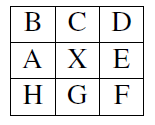
\includegraphics{superblok.png}
\end{center}

\end{block}


\end{frame}
%---------------------------------------------------------------------------
%---------------------------------------------------------------------------
\begin{frame}
\frametitle{Metody przestrzenne}
\begin{block}{Końcowa rekonstrukcja tła}
Dopóki tło nie zostanie w całości uzupełnione
\begin{enumerate}
\item Przesuń ramkę superbloku o jedną pozycję 
\item Sprawdź, czy w superbloku są 3 bloki posiadające tło
\item Jeśli tak, wykonaj transformatę i oblicz funkcję kosztu na 2 wersjach superbloku:
	\begin{enumerate}
	\item Ustaw blok z nieznanym tłem na zero (biała ramka)
	\item Ustaw bloki ze znanym tłem na zero i podstawiaj do nieznanego bloku kolejnych kandydatów
	\end{enumerate}
\item Wstaw w brakujące miejsce blok o najniższym koszcie

\end{enumerate}

\end{block}


\end{frame}
%---------------------------------------------------------------------------
\begin{frame}
\frametitle{Metody przestrzenne}
\begin{block}{Funkcja kosztu}
  \begin{equation}
  \label{costfun}
  cost(k)=\left(\sum_{v=0}^{M-1}\sum_{u=0}^{M-1}\left|C(v,u)+D_k(v,u)\right|\right)\lambda_k
  \end{equation}
  \begin{equation}
  \lambda_k=e^{-\alpha\omega_k}
  \end{equation}
   \begin{equation}
  a\in\langle0,1\rangle
   \end{equation} 
   \begin{equation}
  \omega_k=\frac{W_k}{\sum_{k=0}^{L-1}W_k}
   \end{equation} 
   $W_k$ - waga elementu $r_k$,
   L  - ilość elementów zbioru $r_k$, $C(v,u0)$ - wynik transformaty nr 1, $D_k(v,u)$ - wynik transformaty nr 2 na elemencie k ze zbioru kandydatów
\end{block}


\end{frame}
%---------------------------------------------------------------------------
\begin{frame}
\frametitle{Metody przestrzenne}
\begin{block}{Transformata DCT}
\begin{equation}
X_{k1,k2}=\sum_{n_1=0}^{N_1-1}\sum_{n_2=0}^{N_2-1}x_{n_1,n_2}\cos\left[\frac{\pi}{N_1}\left(n_1+\frac{1}{2}\right)k_1\right]\cos\left[\frac{\pi}{N_2}\left(n_2+\frac{1}{2}\right)k_2\right]
\end{equation}
\end{block}


\end{frame}
%---------------------------------------------------------------------------
\begin{frame}
\frametitle{Metody przestrzenne}
\begin{block}{Transformata Hadamarda}
 \begin{equation}
    H_1=\left[1\right] 
    \end{equation}
    \begin{equation}
           H_2N=\begin{bmatrix}
           H_N&H_N \\
           H_N&-H_N \\
           \end{bmatrix}
    \end{equation}
       \begin{equation}
       F=MXM
       \end{equation}
          \begin{equation}F=
          \begin{bmatrix}
          H& H\\
          H & -H
          \end{bmatrix}
          \begin{bmatrix}
          A& B\\
          C& D
          \end{bmatrix}
             \begin{bmatrix}
             H& H\\
             H & -H
             \end{bmatrix}
          \end{equation}


\end{block}


\end{frame}
%---------------------------------------------------------------------------
\begin{frame}
\begin{center}
\Huge{Metody operujące na pikselach}
\end{center}


\end{frame}

%---------------------------------------------------------------------------

\begin{frame}
\frametitle{Metody operujące na pikselach}
\begin{block}{Założenia}
\begin{itemize}
\item Obliczenia są wykonywane dla pojedynczych pikseli
\item Najczęściej proste algotrymy
\item Wybieranie piksela należącego do tła uzależnione jest od odpowiednich algorytmów
\end{itemize}
\end{block}


\end{frame}
%---------------------------------------------------------------------------

\begin{frame}
\frametitle{Metody operujące na pikselach}
\begin{block}{Właściwości}
\begin{itemize}
\item Najczęściej nie uwzględniają właściwości swojego otoczenia
\item Często możliwe jest wykonywanie w czasie rzeczywistym
\end{itemize}
\end{block}


\end{frame}
%---------------------------------------------------------------------------

\begin{frame}
\frametitle{Metody operujące na pikselach}
\begin{block}{Podział}
\begin{itemize}
\item Metody wykorzysujące bufor
\item Metody bezbuforowe
\end{itemize}
\end{block}


\end{frame}
%---------------------------------------------------------------------------

\begin{frame}
\frametitle{Metody operujące na pikselach}
\begin{block}{Metody wykorzysujące bufor}
\begin{itemize}
\item Bufor zawiera określoną ilość ramek
\item Tło jest obliczane na podstawie kombinacji wielu ramek
\end{itemize}
\end{block}


\end{frame}
%---------------------------------------------------------------------------

\begin{frame}
\frametitle{Metody operujące na pikselach}
\begin{block}{Metoda średniej kroczącej}
\begin{itemize}
\item Wartość piksela tła obliczana jest jako średnia z bufora
\item Możliwe wprowadzenie wag dla poszczególnych ramek
\end{itemize}
\end{block}


\end{frame}
%---------------------------------------------------------------------------

\begin{frame}
\frametitle{Metody operujące na pikselach}
\begin{block}{Metoda średniej kroczącej}
\begin{columns}
\column{0.45\textwidth}
\begin{block}{Zalety}
\begin{itemize}
\item Prosty algorytm
\end{itemize}
\end{block}
\column{0.45\textwidth}
\begin{block}{Wady}
\begin{itemize}
\item Mała dokładność
\item Duża ilość obliczeń czy większych buforach
\end{itemize}
\end{block}
\end{columns}
\end{block}




\end{frame}
%---------------------------------------------------------------------------











\begin{frame}
\frametitle{Metody operujące na pikselach}
\begin{block}{Metody bezbuforowe}
\begin{itemize}
\item Brak bufora
\item Tło jest obliczane na podstawie podstawie obecnej ramki i tła
\end{itemize}
\end{block}


\end{frame}
%---------------------------------------------------------------------------

\begin{frame}
\frametitle{Metody operujące na pikselach}
\begin{block}{Metoda wykorzystująca parametr alfa}
\begin{itemize}
\item Wartość piksela tła obliczana jest jako średnia ważona tła z obecną ramką
\end{itemize}
\end{block}


\end{frame}
%---------------------------------------------------------------------------

\begin{frame}
\frametitle{Metody operujące na pikselach}
\begin{block}{Wartość piksela tła}
  \begin{equation}
  \label{alpha}
  B_{n} = F_{n} * \alpha + B_{n-1} * (1-\alpha)
  \end{equation}
  $B_n$ - wartość piksela tła,\newline
  $F_n$ - wartość piksela obecnej ramki,\newline
  $B_{n-1}$ - poprzednia wartość piksela tła  
\end{block}


\end{frame}
%---------------------------------------------------------------------------

\begin{frame}
\frametitle{Metody operujące na pikselach}
\begin{block}{Metoda wykorzystująca parametr alfa}
\begin{columns}
\column{0.45\textwidth}
\begin{block}{Zalety}
\begin{itemize}
\item Prosty algorytm
\item Bardzo mała ilość obliczeń (mnożenie + dodawanie)
\end{itemize}
\end{block}
\column{0.45\textwidth}
\begin{block}{Wady}
\begin{itemize}
\item Mała dokładność
\end{itemize}
\end{block}
\end{columns}
\end{block}




\end{frame}
%---------------------------------------------------------------------------












\begin{frame}
\frametitle{Metody operujące na pikselach}
\begin{block}{Metoda Mixture of Gaussians \(MOG\)}
\begin{itemize}
\item Oparta o rozkład prawdopodobieństwa Gaussa
\item Piksel należy do tła jeśli spełnia warunek przynależności do jednego z rozkładów
\item Warunkiem przynależności jest wartość w zakresie do 2,5 odchylenia standardowego z danego rozkładu
\end{itemize}
\end{block}

\end{frame}




%---------------------------------------------------------------------------


\begin{frame}
\frametitle{Metody operujące na pikselach}
\begin{block}{Metoda Mixture of Gaussians \(MOG\)}
\begin{columns}
\column{0.45\textwidth}
\begin{block}{Zalety}
\begin{itemize}
\item Dobre rezultaty pracy
\item Złożoność obliczeniowa pozwalająca na pracę w czasie rzeczywistym
\end{itemize}
\end{block}
\column{0.45\textwidth}
\begin{block}{Wady}
\begin{itemize}
\item Bardzo skomplikowany algorytm
\end{itemize}
\end{block}
\end{columns}
\end{block}




\end{frame}
%---------------------------------------------------------------------------

\begin{frame}

\begin{center}

\Huge{Dziękujemy za uwagę}
\end{center}
\end{frame}


\end{document}

